
\section{Parallelizing building neighbor lists}

\begin{frame}{Effects on runtime}{Parallelizing building neighbor lists}


program output on runtimes of different parts

\begin{itemize}
\tightlist
\item
  A40:

  \begin{itemize}
  \tightlist
  \item
    Before:~\texttt{TOTAL\ 3.46s\ FORCE\ 0.21s\ NEIGH\ 3.14s\ REST\ 0.12s}
  \item
    After:~~~~\texttt{TOTAL\ 0.37s\ FORCE\ 0.21s\ NEIGH\ 0.06s\ REST\ 0.09s}
  \end{itemize}
\item
  A100:

  \begin{itemize}
  \tightlist
  \item
    Before:~\texttt{TOTAL\ 3.01s\ FORCE\ 0.05s\ NEIGH\ 2.84s\ REST\ 0.12s}
  \item
    After:~~~~\texttt{TOTAL\ 0.18s\ FORCE\ 0.05s\ NEIGH\ 0.04s\ REST\ 0.10s}
  \end{itemize}
\end{itemize}

As expected we see the runtime spent in the neighborhood computation
drop significantly

With such a reduction in runtime the performance has obviously
increased:

\begin{itemize}
\tightlist
\item
  A40:

  \begin{itemize}
  \tightlist
  \item
    Before:~\texttt{Performance:\ 7.59\ million\ atom\ updates\ per\ second}
  \item
    After:~~~~\texttt{Performance:\ 71.79\ million\ atom\ updates\ per\ second}
  \end{itemize}
\item
  A100

  \begin{itemize}
  \tightlist
  \item
    Before:~\texttt{Performance:\ 7.93\ million\ atom\ updates\ per\ second}
  \item
    After:~~~~\texttt{Performance:\ 143.60\ million\ atom\ updates\ per\ secon}
  \end{itemize}
\end{itemize}

Apart from the reduction in runtime we see also, that the traffic
between device and host has decreased from:

\begin{verbatim}
Total       Count   Avg         Min         Max         Operation
1,36 GiB    229     6,08 MiB    128 B       50,00 MiB   [CUDA memcpy HtoD]
660,00 MiB  220     3,00 MiB    3,00 MiB    3,00 MiB    [CUDA memcpy DtoH]
\end{verbatim}

to:

\begin{verbatim}
Total       Count   Avg         Min         Max         Operation
881,28 MiB  240     3,67 MiB    128 B       4,12 MiB    [CUDA memcpy HtoD]
660,00 MiB  231     2,86 MiB    4 B         3,00 MiB    [CUDA memcpy DtoH]
44 B        11      4 B         4 B         4 B         [CUDA memset]
\end{verbatim}

With this the scaling behaviour also improves:

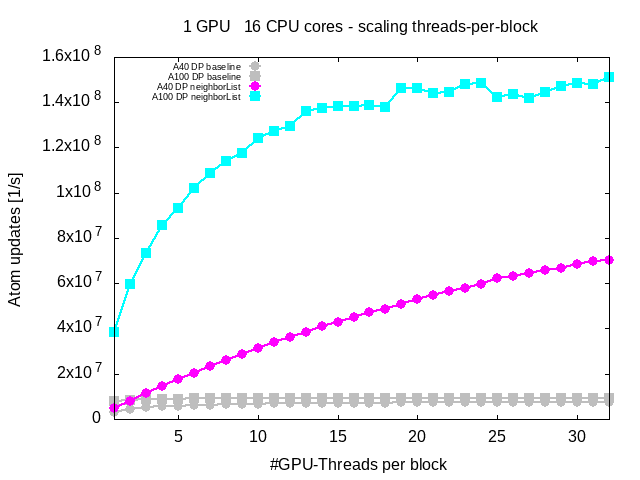
\includegraphics{../resources/development_stage_comparisons/t200_DP_scaling_comparisons/plot_upto_buiNeiPar.png}

\end{frame}



\begin{frame}{Parallelizing further components}

Next we parallelize the updatePbc method which updates the positions of
all ghost atoms. With the parallelization of this method the runtime
drops even further. The reason for this is probably that the full loop
except neighborhood computation now runs on the GPU. This further
improves scaling with threads per block.

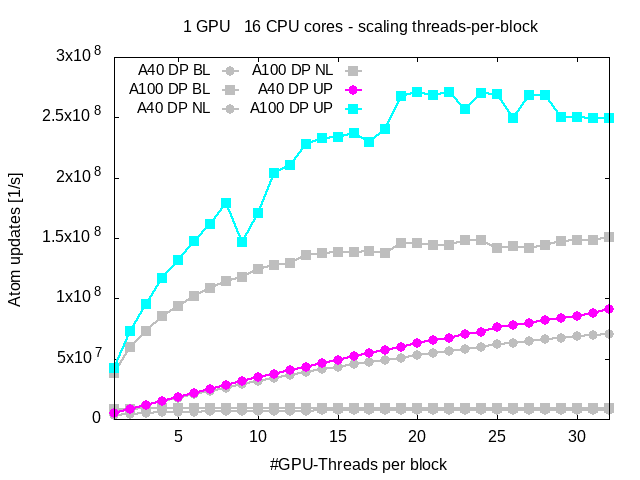
\includegraphics{../resources/development_stage_comparisons/t200_DP_scaling_comparisons/plot_upto_pbcPar.png}

As is visible there is a moderate increase in performance for the A40
and a massive one for the A100. After that the binning of the atoms is
ported to the GPU with only a small increase in performance:

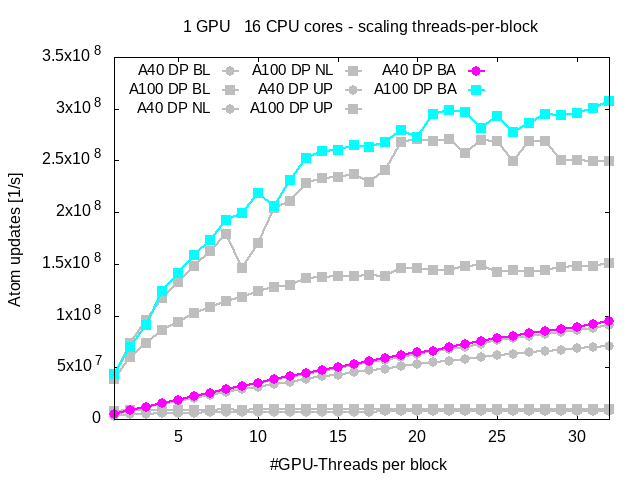
\includegraphics{../resources/development_stage_comparisons/t200_DP_scaling_comparisons/plot_upto_binAtPar.png}

After that the updateAtomsPbc method is ported. This method enforces the
boundary condition on atoms that have left the simulation domain after
the last reneighboring.

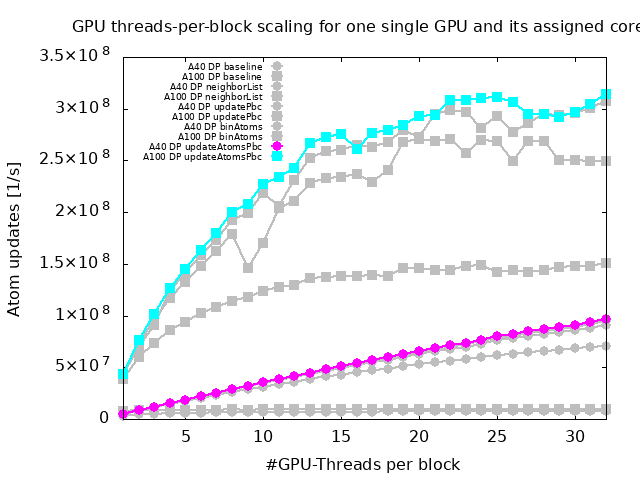
\includegraphics{../resources/development_stage_comparisons/t200_DP_scaling_comparisons/plot_upto_upAtPar.png}

The high variance exhibited in those scaling comparisons is due to the
very low runtimes of the program:

Runtimes with 131072 particles for 200 timesteps:

\begin{itemize}
\tightlist
\item
  A40:
\end{itemize}

\begin{verbatim}
TOTAL 0.27s FORCE 0.21s NEIGH 0.05s REST 0.01s
\end{verbatim}

\begin{itemize}
\tightlist
\item
  A100:
\end{itemize}

\begin{verbatim}
TOTAL 0.09s FORCE 0.05s NEIGH 0.03s REST 0.01s
\end{verbatim}

\end{frame}

\begin{frame}{Whole application scaling behaviour after parallelizing}

Due to those very low runtimes the number of timesteps are now increased
from 200 to 2000 in order to reduce unwanted fluctuations. Additionally
a larger domain size with up to 1048576 atoms (instead of before 131072)
is tested.

The runtimes for default runs (32 threads per block) are now:

\begin{itemize}
\tightlist
\item
  A40:
\end{itemize}

\begin{verbatim}
System: 1048576 atoms 173434 ghost atoms, Steps: 2000
TOTAL 19.57s FORCE 15.49s NEIGH 3.15s REST 0.93s
\end{verbatim}

\begin{itemize}
\tightlist
\item
  A100:
\end{itemize}

\begin{verbatim}
System: 1048576 atoms 173434 ghost atoms, Steps: 2000
TOTAL 4.27s FORCE 2.14s NEIGH 1.54s REST 0.59s
\end{verbatim}

With this the force computation is the main bottleneck. A look into the
cuda profiler confirms this:

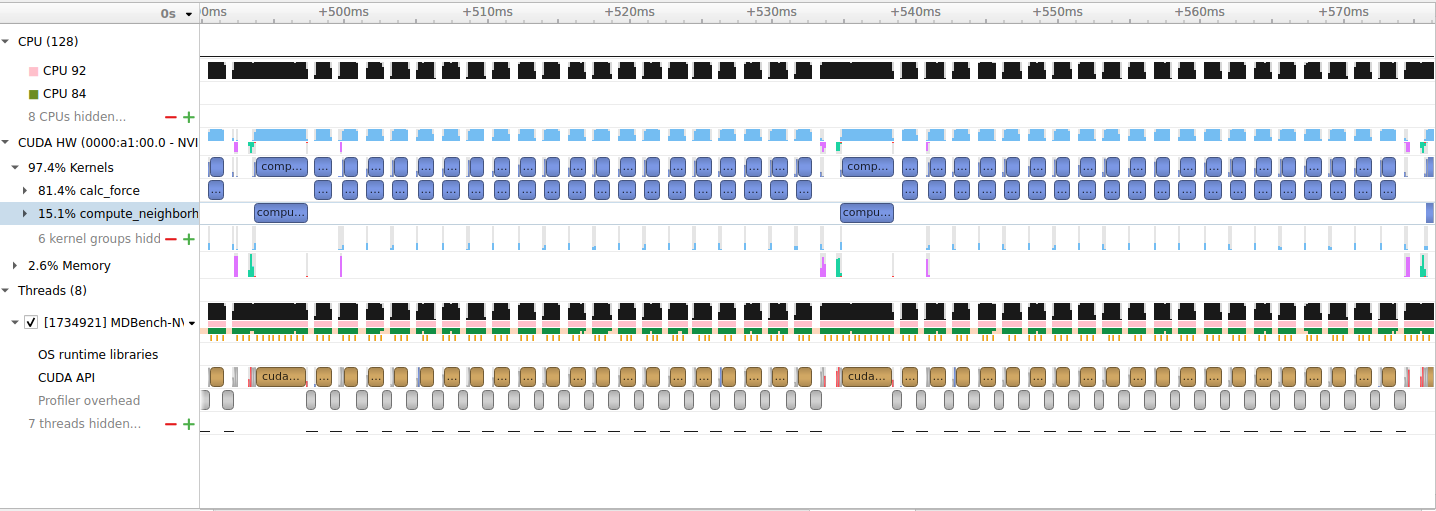
\includegraphics{../resources/profiling/nsys/a40_upAt_profile.png}

However memory transfers still take some time:

\begin{verbatim}
Time     Total Time Count   Min       Max          Operation
67.0%   310,648 ms  523 1,344 μs    475,849 μs  [CUDA memcpy DtoH]
32.0%   150,418 ms  613 1,023 μs    411,571 μs  [CUDA memcpy HtoD]
0.0%    519,530 μs  307   991 ns    898 ns    [CUDA memset]
\end{verbatim}

In the case of the A40 with a runtime of \textasciitilde{}19.5 seconds
this is not a significant portion. For the A100 with a total runtime of
\textasciitilde{}4.3 seconds this represents \textasciitilde{}10.8\% of
the total program runtime.
\end{frame}

\begin{frame}{Runtime spent in the neighbor computation}

In order to find hotspots in the neighborhood computation we instrument
the neighborhood calculation with timestamps. The runtime spent is
summed up over all timesteps for each section and then printed. For the
A40 we get a result like this:

\begin{verbatim}
NEIGH_TIMERS: 
UPD_AT: 0.10s 
SETUP_PBC 0.57s 
UPDATE_PBC 0.20s 
BINATOMS 0.02s 
BUILD_NEIGHBOR 2.31s
\end{verbatim}

\end{frame}

\begin{frame}{Scaling beyond 32 threads per block}

Up to now only scaling until 32 GPU-threads per block have been
examined. However the scaling trend might now continue further than
before the porting. Therefore the next test does scale the amout of
threads exponentially by a factor of 2 from 32 to 1024. Additionally we
take different sizes for the number of atoms to find out, whether the
program with the new neighborhood calculation still operates at max
capacity with the the initial of size of 131072 atoms.

\begin{itemize}
\tightlist
\item
  A40:
\end{itemize}

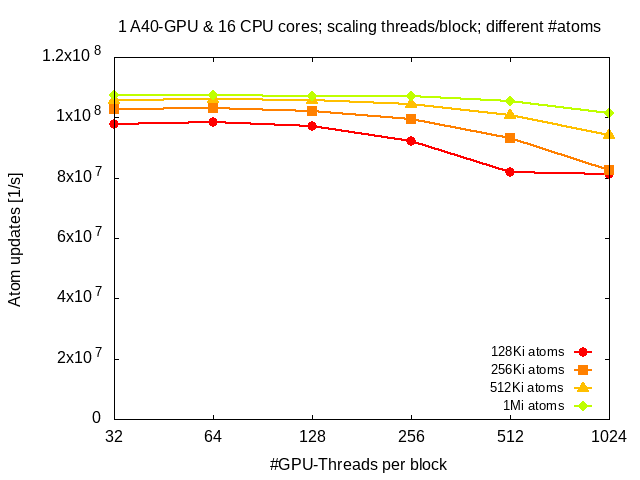
\includegraphics{../resources/scaling/exponential_thread_scaling/gpu32-1024_t2000_p128K-1M/a40_gpu32-1024_t2000_pScaling.png}

The A40 does not scale well beyond 32 threads per block with performance
even reducing. Increasing the number of atoms in the domains yields only
small performance/throughput gains. The dropoff in performance with
larger numbers of threads per block is less severe for a high number of
atoms in the domain.

\begin{itemize}
\tightlist
\item
  A100
\end{itemize}

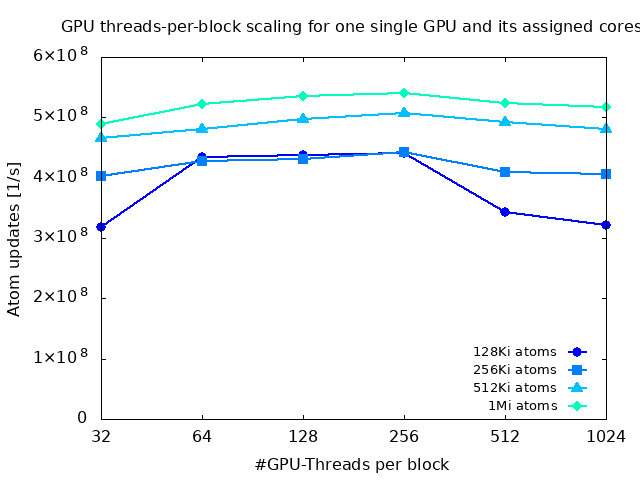
\includegraphics{../resources/scaling/exponential_thread_scaling/gpu32-1024_t2000_p128K-1M/a100_gpu32-1024_t2000_pScaling.png}

The A100 scales much better both with more threads per block and more
atoms in the domain. Around 256 threads per block the maximum seems to
be reached.


\end{frame}

